%%%%%%%%%%%%%%%%%%%%%%%%%%%%%%%%%%%%%%%%
%12pt: grandezza carattere
%a4paper: formato a4
%openright: apre i capitoli a destra
%twoside: serve per fare un documento fronteretro
%report: stile tesi (oppure book)
\documentclass[12pt,a4paper,openany,twoside]{article}

\usepackage[italian]{babel}
%\usepackage[latin1]{inputenc}
\usepackage[utf8]{inputenc}
\usepackage{fancyhdr}
\usepackage{indentfirst}
\usepackage{graphicx}
\usepackage{newlfont}
%librerie matematiche
\usepackage{amssymb}
\usepackage{amsmath}
\usepackage{latexsym}
\usepackage{amsthm}
\usepackage{listings}
\usepackage{chngcntr}
%\usepackage[chapter]{minted}
%librerie per tabelle
\usepackage{tabularx}
\usepackage{threeparttable}

\graphicspath{ {./figures/} }

\oddsidemargin=30pt \evensidemargin=20pt%impostano i margini
\hyphenation{sil-la-ba-zio-ne pa-ren-te-si}

\usepackage[square, numbers, comma, sort&compress]{natbib} %Bibliografia
\usepackage{hyperref}
\usepackage{float}

\usepackage[pass]{geometry}

%comandi per l'impostazione della pagina, vedi il manuale della libreria fancyhdr per ulteriori delucidazioni
\pagestyle{fancy}\addtolength{\headwidth}{20pt}
%\renewcommand{\chaptermark}[1]{\markboth{\thechapter.\ #1}{}}
\renewcommand{\sectionmark}[1]{\markright{\thesection \ #1}{}}
\rhead[\fancyplain{}{\bfseries\leftmark}]{\fancyplain{}{\bfseries\thepage}}
\cfoot{}

\linespread{1.3} %comando per impostare l'interlinea

%\renewcommand{\listingscaption}{Codice}
%\renewcommand{\listoflistingscaption}{Elenco dei Codici}

\begin{document}
%%%%%%%%%%%%%%%%%%%%%%%%%%%%%%%%%%%%%%%%
% FRONTESPIZIO
\newgeometry{hmarginratio=1:1}
\begin{titlepage}
\begin{center}
%\includegraphics[width=2.56in]{figures/logo/logo_unibo.png}\\
% {{\Large{\textsc{Alma Mater Studiorum $\cdot$ Universit\`a di
% Bologna}}}} \rule[0.1cm]{14.7cm}{0.1mm}
% \rule[0.5cm]{14.7cm}{0.6mm}
%\vspace{5mm}
{\small{\bf SCUOLA DI INGEGNERIA E ARCHITETTURA\\
\vspace{2mm}
Dipartimento di Informatica -- Scienza e Ingegneria\\
\vspace{2mm}
Corso di Laurea Magistrale in Ingegneria Informatica }}
%se Laurea Magistrale scrivere "Corso di Laurea Magistrale in Ingegneria Informatica"
\end{center}
%\vspace{11.9mm}

\vspace*{\fill}
\begin{center}
{\LARGE{\bf Simulazione di Fluidi in CUDA\\
\vspace{5mm}
}}
\end{center}
%\vspace{11.9mm}
\vspace*{\fill}
\par
\noindent
\vfill
\begin{minipage}[t]{0.47\textwidth}
{\normalsize{\bf Professori:\\
Prof. Dr. Stefano Mattoccia \\
Prof. Dr. Fabio Tosi

%\vspace{5mm}
%Correlatori:\\
%Dr. Antonio Iacobelli\\
}}
\end{minipage}
\hfill
\begin{minipage}[t]{0.47\textwidth}\raggedleft
{\normalsize{\bf Presentata da:\\
Enrico Minguzzi}}
\end{minipage}
\vspace{10mm} % da aumentare a 20 o 30 se non si inseriscono i correlatori
\begin{center}
{\normalsize{%\bf Sessione \\%inserire il numero della sessione in cui ci si laurea
Anno Accademico 2024-2025}}%inserire l'anno accademico a cui si è iscritti
\end{center}
\end{titlepage}

\restoregeometry

%%%%%%%%%%%%%%%%%%%%%%%%%%%%%%%%%%%%%%%%
% INDICE 
%\tableofcontents %crea l'indice
%imposta l'intestazione di pagina
%\rhead[\fancyplain{}{\bfseries\leftmark}]{\fancyplain{}{\bfseries\thepage}}
%\lhead[\fancyplain{}{\bfseries\thepage}]{\fancyplain{}{\bfseries
%Indice}}



%%%%%%%%%%%%%%%%%%%%%%%%%%%%%%%%%%%%%%%%
% ELENCO DELLE FIGURE
%\clearpage{\pagestyle{empty}\cleardoublepage}
%\renewcommand{\listfigurename}{Elenco delle Figure}
%\phantomsection
%\addcontentsline{toc}{chapter}{Elenco delle Figure}
%\listoffigures %crea l'elenco delle figure



%%%%%%%%%%%%%%%%%%%%%%%%%%%%%%%%%%%%%%%%
% ELENCO DELLE TABELLE
%\clearpage{\pagestyle{empty}\cleardoublepage}
%\renewcommand{\listtablename}{Elenco delle Tabelle}
%\phantomsection
%\addcontentsline{toc}{chapter}{Elenco delle Tabelle}
%\listoftables %crea l'elenco delle tabelle


%%%%%%%%%%%%%%%%%%%%%%%%%%%%%%%%%%%%%%%%
% ELENCO DEI CODICI
%\clearpage{\pagestyle{empty}\cleardoublepage}
%\phantomsection
%\addcontentsline{toc}{chapter}{Elenco dei Codici}
%\listoflistings %crea l'elenco dei codici


%%%%%%%%%%%%%%%%%%%%%%%%%%%%%%%%%%%%%%%%
% INTRODUZIONE
%\clearpage{\pagestyle{empty}\cleardoublepage}
%\chapter{Introduzione} 
%\lhead[\fancyplain{}{\bfseries\thepage}]{\fancyplain{}{\bfseries\rightmark}}
%\pagenumbering{arabic} %mette i numeri arabi

%\clearpage{\pagestyle{empty}\clearpage}



%%%%%%%%%%%%%%%%%%%%%%%%%%%%%%%%%%%%%%%%
% STUDIO DEL PROBLEMA
\section{Studio del Problema}
%Iniziare con un’analisi dettagliata del problema da risolvere. Questa fase deve
%includere lo studio della natura dei dati in input e output, la comprensione
%delle operazioni computazionali richieste e l’identificazione delle dipendenze
%tra i dati. Questa fase preliminare `e cruciale per comprendere se e come il pro-
%blema possa beneficiare della parallelizzazione su GPU, identificare eventuali
%limitazioni o criticit`a intrinseche e definire una strategia iniziale di decom-
%posizione del problema. Le considerazioni fatte in questa fase guideranno le
%scelte implementative successive.
\subsection{Introduzione}

%One of the most intriguing problems in computer graphics is the simulation of fluid-like behavior. A good fluid solver is of great importance in many different areas. In the special effects industry there is a high demand to convincingly mimic the appearance and behavior of fluids such as smoke, water and fire. Paint programs can also benefit from fluid solvers to emulate traditional techniques such as watercolor and oil paint. Texture synthesis is another possible application. Indeed, many textures result from fluid-like processes, such as erosion. The modeling and simulation of fluids is, of course, also of prime importance in most scientific disciplines and in engineering. Fluid mechanics is used as the standard mathematical framework on which these simulations are based

Uno dei problemi più affascinanti nell'ambito della computer graphics è la simulazione del comportamento dei fluidi \cite{abbott1989computational, 10.1145/311535.311548, fernando2004gpu, chorin2013mathematical}. Un buon \textit{fluid solver} (simulatore di fluidi) riveste grande importanza in molti settori diversi. Nell'industria degli effetti speciali, ad esempio, esiste una grande richiesta di riprodurre in modo convincente l'aspetto e il comportamento di fluidi come fumo, acqua e fuoco. Anche i programmi di pittura digitale possono trarre vantaggio dai \textit{fluid solver} per emulare tecniche tradizionali come l'acquerello e la pittura a olio. Un'altra possibile applicazione è la sintesi delle texture: molti motivi, infatti, derivano da processi fluidodinamici, come l'erosione. La modellazione e la simulazione dei fluidi sono, ovviamente, fondamentali anche nella maggior parte delle discipline scientifiche e nell'ingegneria. A fornire il quadro matematico standard su cui si basano queste simulazioni è la meccanica dei fluidi.
Nella comunità scientifica vi è consenso sul fatto che le equazioni di \textbf{Navier-Stokes} costituiscano un modello estremamente accurato per descrivere il flusso dei fluidi. Migliaia di libri e articoli sono stati pubblicati in vari ambiti su come calcolare numericamente queste equazioni. La scelta del \textit{solver} da utilizzare nella pratica dipende in larga misura dal problema specifico e dalla potenza di calcolo disponibile.

Il modello preso in considerazione da questo progetto non è sufficientemente accurato per la maggior parte delle applicazioni ingegneristiche. Infatti, presentando un eccesso di “dissipazione numerica”, il flusso tende a smorzarsi troppo rapidamente rispetto a quanto osservato negli esperimenti reali. In un’applicazione nell'ambito della computer graphics, questo non rappresenta un problema così grave, specialmente in un sistema interattivo dove il flusso viene “tenuto vivo” da un animatore che applica forze esterne. In effetti, un flusso che non si smorza affatto potrebbe risultare troppo caotico e difficile da controllare.

Nella seguente sezione vengono presentate le equazioni di \textbf{Navier-Stokes} e le relative considerazioni per l'implementazione svolta.

\section{Equazioni di Navier-Stokes}
La simulazione proposta si basa sull'ipotesi di un fluido incomprimibile contenuto in un dominio quadrato bidimensionale, rappresentato da una griglia quadrata composta da celle \cite{fernando2004gpu, 10.1145/311535.311548}.

Il componente centrale di qualsiasi \textit{fluid solver} è costituito da un risolutore numerico per le equazioni di Navier-Stokes, specifiche per un flusso incomprimibile \cite{chorin2013mathematical}:
\begin{align*}
	&\frac{\partial \vec{u}}{\partial t} = - (\vec{u} \cdot \nabla) \vec{u} - \frac{1}{\rho} \nabla p + \nu \nabla^2 \vec{u} + \vec{F} \\
	&\nabla \cdot \vec{u} = 0
\end{align*}
dove \(\vec{x} = (x,y)\) sono le coordinate spaziali, \(t\) rappresenta la variabile temporale, \(\vec{u}(\vec{x},t)\) è il campo vettoriale della velocità, \(p(\vec{x},t)\) è il campo scalare della pressione, \(\rho\) è la densità costante del fluido, \(\nu\) è la viscosità dinamica, e \(\vec{F} = (f_x,f_y)\) rappresenta le forze esterne che agiscono sul fluido.

Il risolutore calcola iterativamente il comportamento del fluido: ad ogni iterazione, o time step, un insieme discreto di operatori differenziali viene applicato a un piccolo gruppo di celle nel dominio. Questi operatori aggiornano lo stato del fluido, come la velocità e la pressione, basandosi sui valori della griglia computati al time step precedente. 
Per questa implementazione, un'iterazione consiste nel calcolo di diversi termini:

\begin{itemize}
    \item \textbf{Forze esterne} - Questo termina incorpora l'accelerazione generata da forze applicate al fluido. Queste forze possono essere forze locali o forze globali. Le forze locali si applicano a una regione specifica del fluido, ad esempio un ventilatore che soffia aria su un'area circoscritta. Al contrario, le forze globali, come la forza di gravità, si applicano uniformemente all'intero fluido. Nell'implementazione proposta, le forze esterne vengono inizializzate con valori casuali e utilizzate solo nella prima iterazione per semplicità
    \item \textbf{Avvezione} - La velocità del fluido causa il trasporto di quantità come densità, coloranti o altre proprietà lungo il flusso. Analogamente, anche il fluido stesso trasporta la propria velocità, creando un effetto autotrasportante.
    \item \textbf{Diffusione} - Ogni fluido ha una certa viscosità, che misura la resistenza al movimento. Questa proprietà determina una diffusione del momento (e quindi di velocità), influenzando il comportamento del fluido.
    \item \textbf{Proiezione} - Nei fluidi incomprimibili, il campo di velocità deve essere privo di divergenza. In caso contrario, parti del fluido potrebbero scomparire, rendendo la simulazione inaccurata. Questo passaggio garantisce che il campo di velocità rimanga solenoidale.
\end{itemize}
In un'implementazione tipica, i vari termini non vengono semplicemente calcolati e sommati tra loro, ma la soluzione è ottenuta attraverso la composizione di trasformazioni sullo stato del fluido. In altre parole, ogni componente può essere visto come una funzione che riceve un campo come input e produce un nuovo campo come output.
\newline
\newline
I kernel usati in questi passaggi accedono ai dati in modo contiguo per ciascuna cella della griglia. Di conseguenza, gli algoritmi risultano altamente parallelizzabili, rappresentando un ottimo esempio per l'applicazione del modello di programmazione CUDA. La parallelizzazione del \textit{solver} avviene eseguendo blocchi composti da centinaia di thread distribuiti sull'intero dominio, dove ciascuno di essi applica i kernel a un ristretto numero di celle.

\subsection{Limitazioni}
%identificare eventuali limitazioni o criticit`a intrinseche e definire una strategia iniziale di decomposizione del problema

Le tre limitazioni maggiori nella parallelizzazione di ogni iterazione sono le seguenti:
\begin{itemize}
    \item \textbf{Composizione di Funzioni} - Poiché il risultato è ottenuto tramite una composizione di funzioni, i kernel non sono indipendenti. Questo implica che il kernel \(i\) richiede che il kernel \(i - 1\) abbia completato la sua computazione e, di conseguenza, è necessaria una sincronizzazione (implicita se si sta utilizzando un solo stream) tra di essi.
    \item \textbf{Iterazioni di Jacobi} - Nella implementazione della \textbf{diffusione}, per la risoluzione dell'equazione di Poisson \(\nabla^2 x = b\), si utilizza il metodo iterativo di Jacobi \cite{golub2013matrix}. Tuttavia, questo algoritmo presenta una limitazione legata alla dipendenza tra i blocchi di thread. Si supponga che ogni thread calcoli un singolo elemento e si indichi con \(W\) e \(H\) rispettivamente la larghezza e l'altezza del blocco. Per computare un blocco di dimensione \(W \times H\), è necessario considerare anche le celle dell'anello esterno, indispensabili per calcolare il laplaciano, portando quindi a un blocco effettivo di dimensione \((W + 2) \times (H + 2)\). Se l'iterazione venisse eseguita direttamente nel codice di ciascun thread, quelli posizionati ai bordi del blocco \(i\), che dipendono dai valori esterni al blocco stesso, rischierebbero di leggere dati obsoleti, dovendo essere aggiornati dai thread del blocco \(i + 1\). Questa limitazione comporta la necessità di effettuare multiple chiamate al kernel dal codice host per sincronizzarli implicitamente, aumentando significativamente il tempo di computazione per completare l'intero time step.
    
    %Infatti, supponendo che un thread computi un singolo elemento, detta \(W\) la larghezza e \(H\) l'altezza del blocco, per computare il blocco \(W \times H\) servono anche le celle dell'anello esterno (per calcolare il laplaciano), risultando quindi in un blocco \((W + 2) \times (H + 2)\). %Di conseguenza, il metodo non può essere implementato con una singola chiamata al kernel. 
    %Se l'iterazione fosse eseguita direttamente nel codice di ciascun thread, i thread situati ai confini del blocco \(i\), che richiedono valori al di fuori del blocco stesso, rischierebbero di leggere dati obsoleti e non ancora aggiornati dai thread del blocco \(i + 1\). Questa limitazione comporta la necessità di effettuare multiple chiamate al kernel dal codice host per sincronizzarli implicitamente, aumentando significativamente il tempo di computazione per completare l'intero time step.
    \item \textbf{Avvezione} - Se si utilizza un flusso con valori casuali del campo vettoriale della velocità, le posizioni della griglia calcolate nel metodo semi-Lagrangiano (\emph{backtracking}) per l'interpolazione bilineare sono sparse. Quindi, non avendo un preciso pattern, le richieste di memoria non possono essere rese coalescenti, e l'efficacia delle cache L1 e L2 non può essere sfruttata a pieno.
\end{itemize}

\subsection{Implementazione Sequenziale}
L'implementazione sequenziale di base realizza le funzionalità descritte in precedenza. Per ottimizzare l'efficienza, è stata adottata una strategia che utilizza due puntatori alla griglia: all'interno di una generica funzione, il primo puntatore viene aggiornato, mentre il secondo viene utilizzato come base da cui prelevare i valori. Al termine della funzione, i puntatori vengono scambiati, evitando operazioni ridondanti di copia dei dati. I risultati sperimentali, ottenuti mediando i valori su 50 iterazioni consecutive, sono riportati in Figura \ref{fig:1}.

\begin{figure}
    \centering
    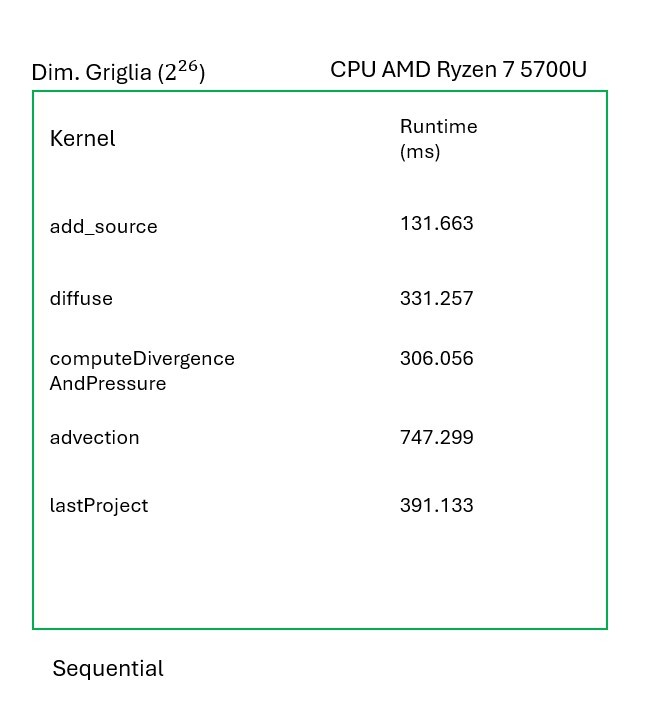
\includegraphics[width=0.5\linewidth]{Slide1-Mod.jpg}
    \caption{Statistiche codice sequenziale}
    \label{fig:1}
\end{figure}

%\clearpage{\pagestyle{empty}\clearpage}



%%%%%%%%%%%%%%%%%%%%%%%%%%%%%%%%%%%%%%%%
% DECOMPOSIZIONE E STRUTTURA PARALLELA
%Definire la strategia di decomposizione del problema identificando le com-
%ponenti parallelizzabili e progettando una struttura parallela di alto livello.
%Questa fase richiede particolare attenzione all’organizzazione gerarchica di
%griglie, blocchi e thread, alla definizione del mapping tra dati e thread, e
%all’identificazione dei pattern di accesso ai dati.
\section{Decomposizione e Struttura Parallela}

\subsection{Descrizione dei Kernel Principali}
In questa sezione vengono illustrati i principali kernel implementati nell'applicazione:
\begin{enumerate}
    \item \textbf{add\_source} - Moltiplica la sorgente per il passo temporale  e somma il risultato al valore preesistente, aggiornando infine il valore sulla griglia.

    \item \textbf{diffuse} - Esegue un'iterazione del metodo di Jacobi. Per il calcolo vengono caricati i valori delle celle adiacenti (destra, sinistra, sopra, sotto) dall'iterazione precedente, moltiplicati per una costante specifica, e sommati al valore centrale iniziale. Questo kernel viene utilizzato per risolvere sia l'equazione di Poisson legata alla diffusione nell'equazione di Navier-Stokes, sia quella per il calcolo della pressione nella fase finale di proiezione.

    \item \textbf{computeDivergenceAndPressure} - Calcola la divergenza del campo vettoriale delle velocità per ogni cella della griglia e inizializza a zero il campo della pressione.

    \item \textbf{advection} - Implementa il trasporto di una quantità (densità o componente di velocità) mediante approccio semi-Lagrangiano con backtracking, garantendo stabilità numerica. La quantità in posizione retro-trasportata viene determinata attraverso interpolazione bilineare dei valori circostanti.

    \item \textbf{lastProject} - Completa la fase di proiezione sottraendo il gradiente del campo di pressione al campo vettoriale delle velocità precedentemente calcolato.

\end{enumerate}


\subsection{Implementazioni Parallele Na{\"i}ve Iniziali}
Per parallelizzare il singolo time step, sono state testate tre strategie di decomposizione della griglia:

\begin{enumerate}
\item \textbf{Decomposizione 1:1} - Ogni thread calcola una singola cella (\texttt{BlockPerElement}).
\textit{Vantaggio}: Accessi alla memoria globalmente coalescenti grazie alla località spaziale dei dati.

\item \textbf{Decomposizione 1:N} - Ogni thread elabora una sottogriglia di \(2^{\texttt{GRID\_DIVISION\_FACTOR}}\) celle (\texttt{BlockPartitioned}).  
\textit{Svantaggio}: Accessi non coalescenti, poiché thread adiacenti operano su regioni distanti della griglia, con possibile riduzione della bandwidth effettiva.

\item \textbf{Decomposizione 1:N} - Ogni thread gestisce \(2^{\texttt{GRID\_DIVISION\_FACTOR}}\) celle distribuite uniformemente sulla griglia (\texttt{Interleaved}).  
\textit{Vantaggio}: Coalescenza degli accessi alla memoria preservata attraverso un pattern di accesso strided.

\end{enumerate}

Nelle Figure \ref{fig:2} \ref{fig:3} \ref{fig:5} sono confrontate le metriche chiave (analizzate con \texttt{Nsight Compute}).

\begin{figure}
    \centering
    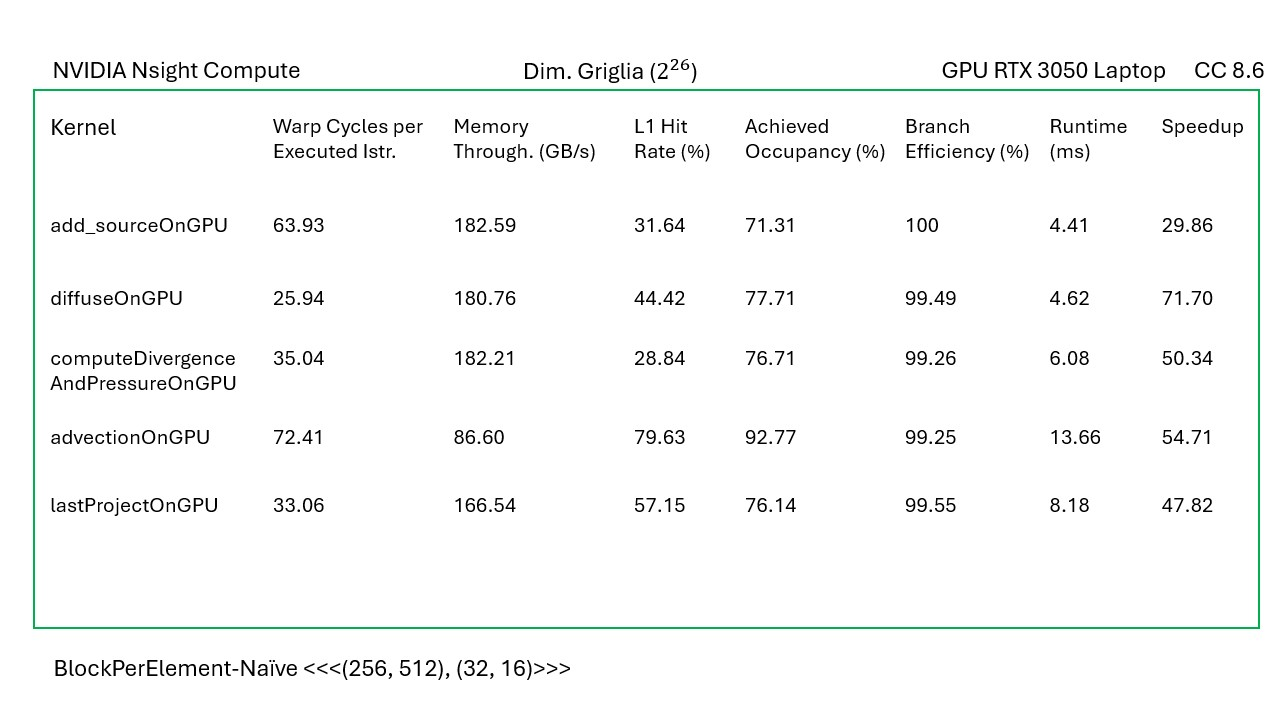
\includegraphics[width=0.75\linewidth]{figures/Slide2.jpg}
    \caption{Statistiche codice parallelo \texttt{BlockPerElement-Naive}}
    \label{fig:2}
\end{figure}

\begin{figure}
    \centering
    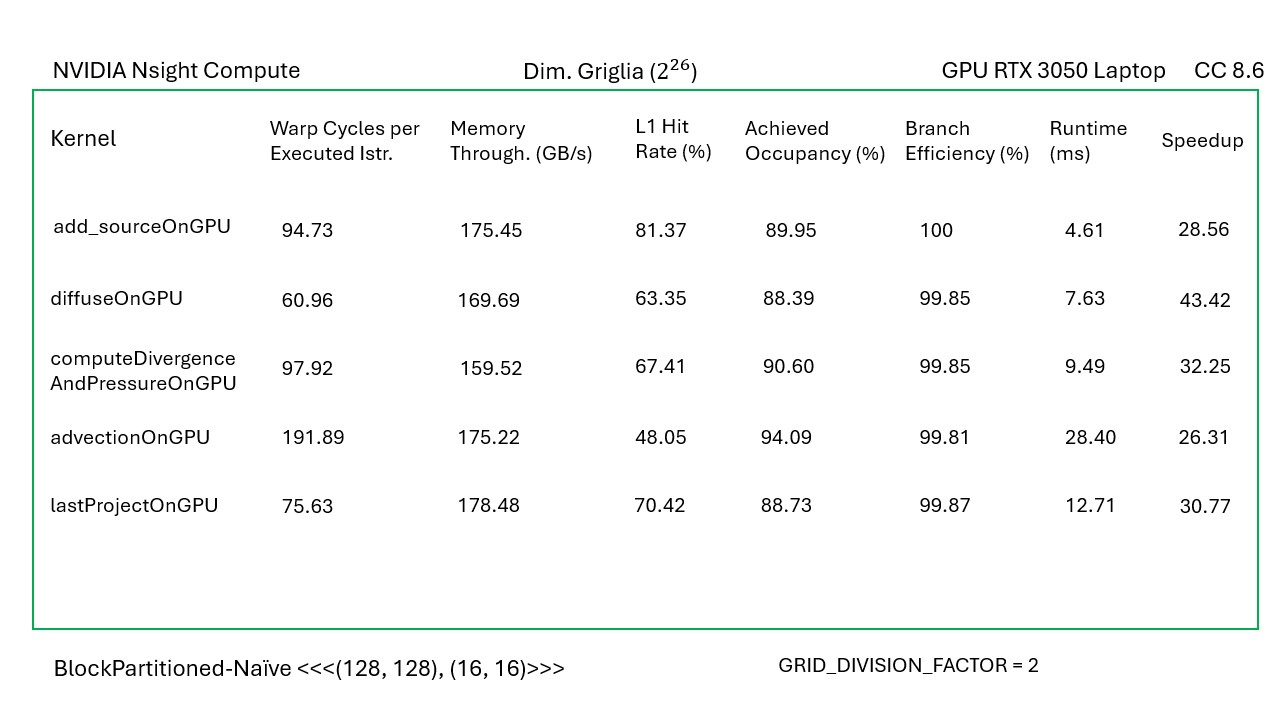
\includegraphics[width=0.75\linewidth]{figures/Slide3.jpg}
    \caption{Statistiche codice parallelo \texttt{BlockPartitioned-Naive}}
    \label{fig:3}
\end{figure}

Per quanto riguarda le versioni \texttt{BlockPerElement} \ref{fig:2} e \texttt{Interleaved} \ref{fig:5}, entrambe raggiungono una Occupancy elevata, con elevati livelli di Memory Throughput e Cache Hit, indicando una corretta parallelizzazione dei vari kernel. Tuttavia, poiché il risultato è ottenuto attraverso una composizione di funzioni, i kernel non possono essere collassati in uno unico, che permetterebbe di utilizzare maggiormente le pipeline di computazione e aumentare il Compute Throughput complessivo. Invece, per quanto riguarda il \texttt{BlockPartitioned} \ref{fig:3}, nonostante l'Hit Rate della Cache L1 sia elevato, in media solo \(7.9\) su \(32\) byte trasmessi per settore sono utilizzati da ogni thread. Questo inefficiente utilizzo della banda di memoria globale è molto probabilmente dovuto al pattern di accesso ai dati.

\begin{figure}
    \centering
    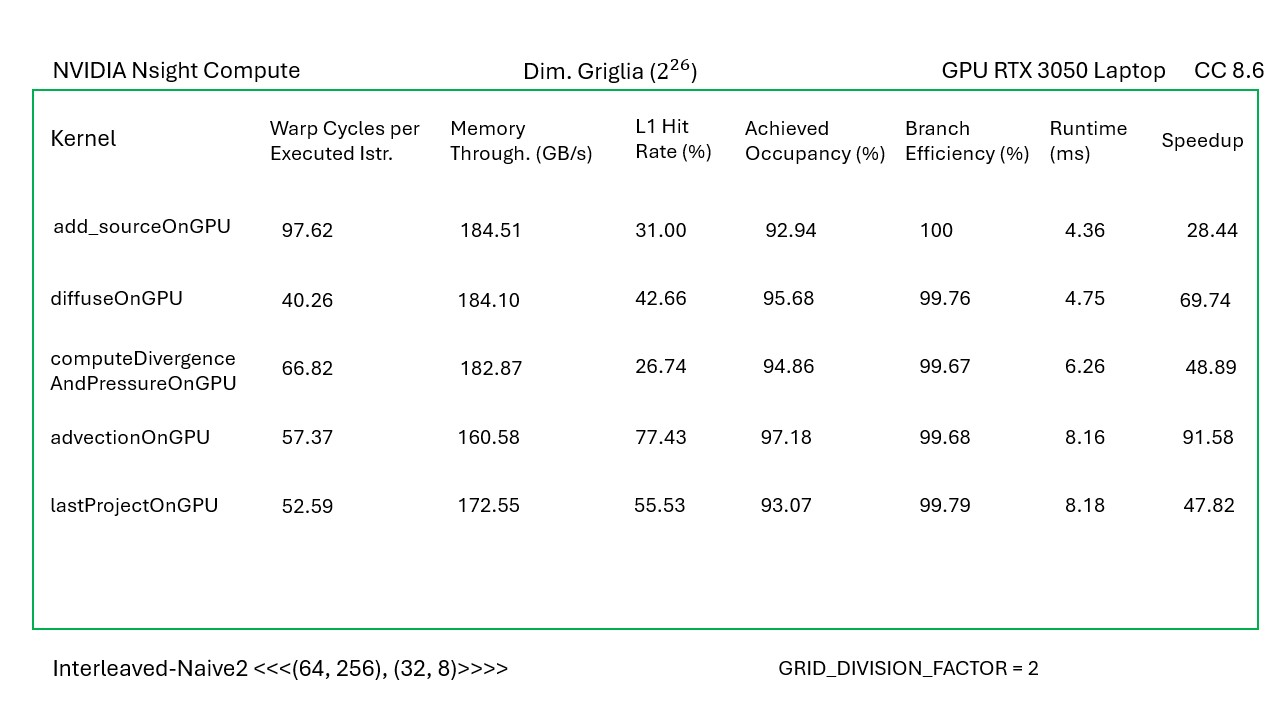
\includegraphics[width=0.75\linewidth]{figures/Slide5.jpg}
    \caption{Statistiche codice parallelo \texttt{Interleaved-Naive2}}
    \label{fig:5}
\end{figure}

Infine, l'analisi del Roofline Model delle varie versioni evidenzia chiaramente la natura memory-bound dei kernel. Tuttavia, il posizionamento sulla Bandwidth Roof suggerisce un ottimo sfruttamento delle risorse computazionali disponibili.

%\clearpage{\pagestyle{empty}\clearpage}



%%%%%%%%%%%%%%%%%%%%%%%%%%%%%%%%%%%%%%%%
% OTTIMIZZAZIONI INCREMENTALI
\section{Ottimizzazioni Incrementali}
%Come abbiamo implementato il programma, se ci sono state scelte particolari o punti particolarmente ostici che sono stati superati. Se ci sono state difficolt\`a insormontabili vanno spiegate.\\
%\`E necessario inserire estratti di codice, tabelle o immagini nella tesi solamente quando questi aiutano la comprensione dell'argomento. Se pensate di stare scrivendo una parte molto tecnica e poco comprensibile al lettore, aiutatevi con le immagini o con il codice. Per inserire estratti di codice rifarsi all'esempio seguente oppure \`e possibile usare il package  \href{https://www.overleaf.com/learn/latex/Code\_listing}{listing}.
%\begin{minted}{c}
%#include <stdio.h>
%int main() {
%   // printf() displays the string inside quotation
%   printf("Hello, World!");
%   return 0;
%}
%\end{minted}

L'analisi delle metriche delle prime versioni parallele evidenzia la scarsa praticabilità di ulteriori miglioramenti utilizzando i metodi inizialmente considerati per affrontare il problema. Tuttavia, si è comunque scelto di sperimentare l'uso della shared memory e della tecnica del loop unrolling, sia come esercizio di ottimizzazione, sia nella prospettiva di possibili sviluppi futuri, qualora le limitazioni iniziali possano essere mitigate.

\subsection{Shared Memory}
\begin{figure}
    \centering
    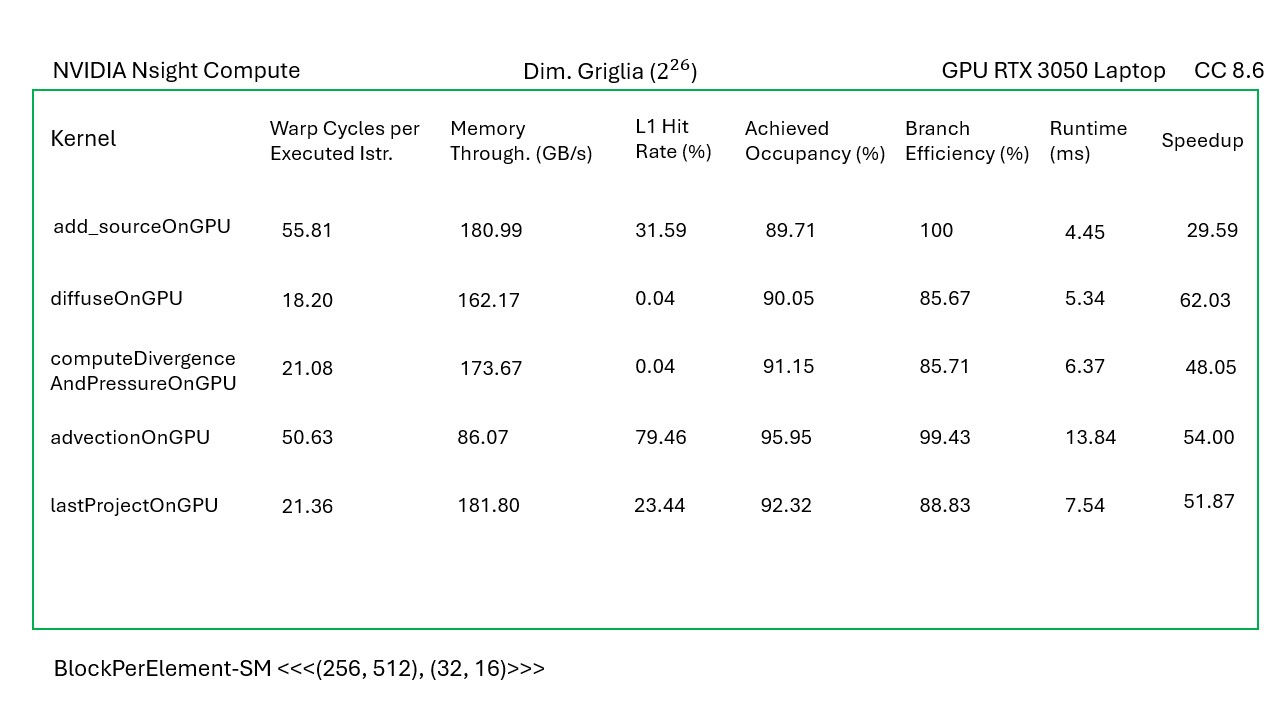
\includegraphics[width=0.75\linewidth]{figures/Slide6.jpg}
    \caption{Statistiche codice parallelo \texttt{BlockPerElement-SM}}
    \label{fig:6}
\end{figure}


\begin{figure} 
    \centering
    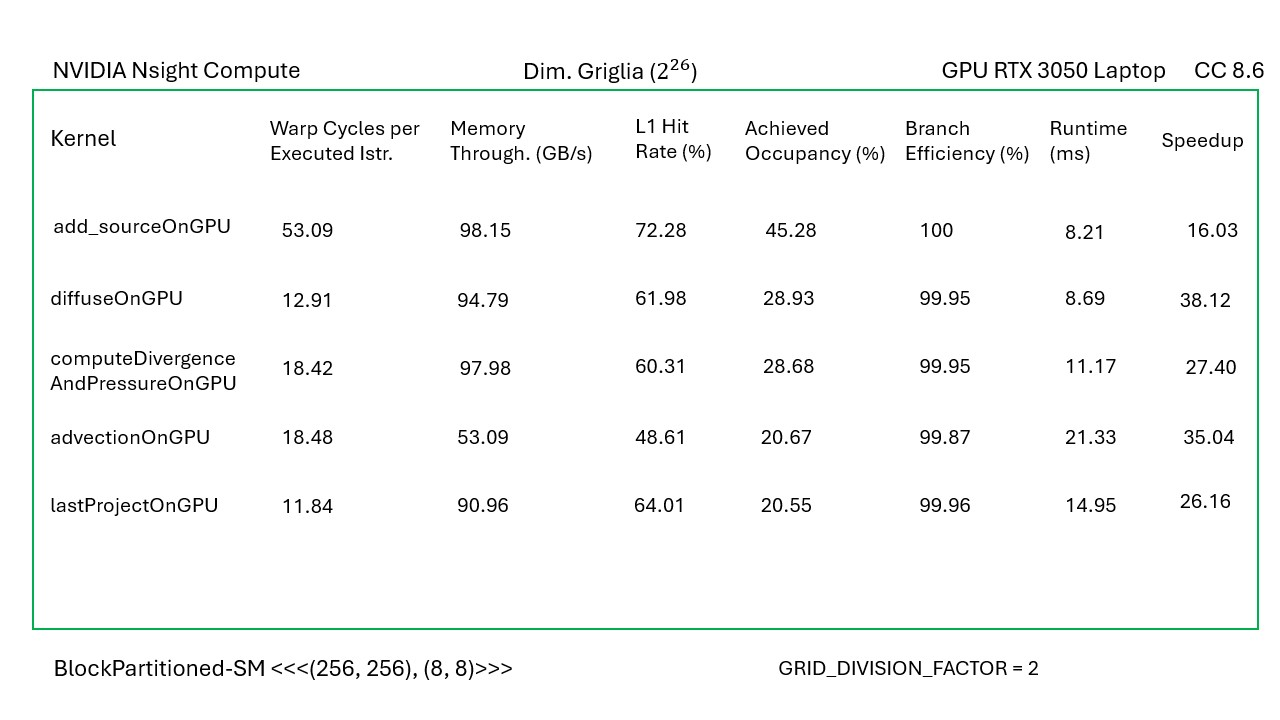
\includegraphics[width=0.75\linewidth]{figures/Slide7.jpg}
    \caption{Statistiche codice parallelo \texttt{BlockPartitioned-SM}}
    \label{fig:7}
\end{figure}

%Per quanto riguarda la versione BlockPerElement-SM \ref{fig:6}, l'utilizzo della shared memory non rende più efficiente il kernel. Questo perché l'overhead iniziale di caricare i dati dalla memoria globale alla shared memory non viene compensato dal resto del codice. Infatti, sia nella versione SM sia in quella Naive, il numero di accessi alla memoria globale rimane invariato. Se i kernel fossero più lunghi e facessero molteplici accessi alla memoria globale, l'utilizzo della shared memory sarebbe giustificato e le perfomance aumenterebbero.
Nella versione \texttt{BlockPerElement-SM} \ref{fig:6}, l'impiego della shared memory non migliora l'efficienza del kernel. Questo perché l'overhead introdotto dal caricamento dei dati dalla memoria globale alla shared memory non viene compensato dalle operazioni successive. Infatti, sia nella versione SM che in quella Na{\"i}ve, il numero di accessi alla memoria globale rimane invariato. L'uso della shared memory sarebbe vantaggioso solo in presenza di kernel più lunghi, con molteplici accessi alla memoria globale, dove il riutilizzo dei dati potrebbe effettivamente tradursi in un miglioramento delle prestazioni.

\begin{figure}
    \centering
    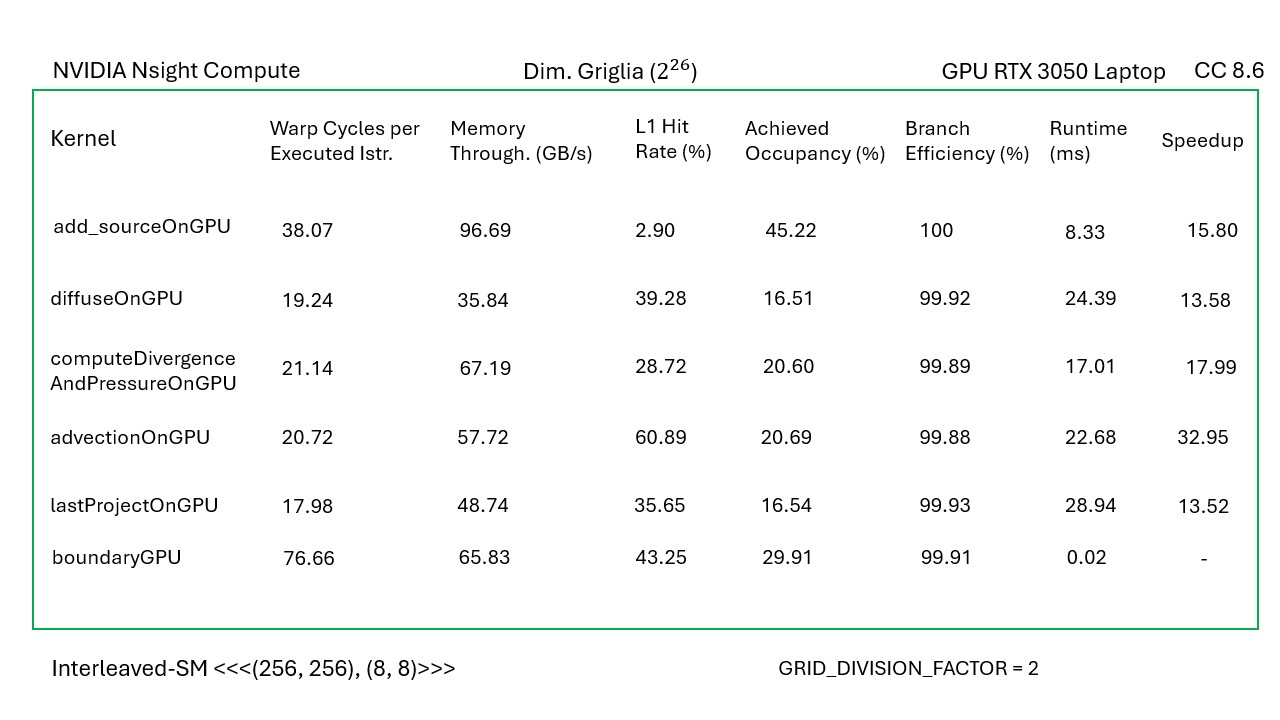
\includegraphics[width=0.75\linewidth]{figures/Slide8.jpg}
    \caption{Statistiche codice parallelo \texttt{Interleaved-SM}}
    \label{fig:8}
\end{figure}

%Nelle altre due versioni \ref{fig:7} \ref{fig:8}, il problema principale è l'Occupancy. Infatti, poiché ogni thread deve computare più di una cella, le dimensioni della shared memory per ogni blocco diventano significative e, aumentando il numero di elementi della griglia, per alcuna configurazioni di lancio dei kernel, possono anche sforare i limiti di shared memory per blocco. Avendo una occpuancy così bassa, il latency hiding non è fattibile, e i tempi di esecuzione sono considerevolemente più lunghi.
Nelle altre due versioni \ref{fig:7} \ref{fig:8}, il principale fattore limitante è l'Occupancy. Poiché ogni thread deve elaborare più di una cella, l'uso della shared memory per blocco diventa significativo e, con l'aumentare delle dimensioni della griglia, alcune configurazioni di lancio dei kernel possono superare i limiti imposti dall'architettura hardware. A causa della bassa Occupancy, il latency hiding diventa inefficace, portando a tempi di esecuzione significativamente più lunghi.

\subsubsection{Cooperative Groups}
Per superare la limitazione dei kernel separati, si è provato a utilizzare i \textit{cooperative groups} per gestire le sincronizzazioni inter-block. Tuttavia, poiché anche essi richiedono grandi quantità di shared memory, se si aumentano le dimensioni della griglia, si rischia di superare il limite di shared memory per blocco.

\subsection{Loop Unrolling}
Come ultima ottimizzazione si è utilizzata la tecnica del loop unrolling \ref{fig:9}. Il loop unrolling viene introdotto per diminuire il sovraccarico delle istruzioni di salto e aumentare l'efficienza delle operazioni parallele, poiché le istruzioni nel ciclo srotolato (unrolled) sono più indipendenti, consentendo alla GPU (e thread CUDA) di eseguirle simultaneamente.

\begin{figure}
    \centering
    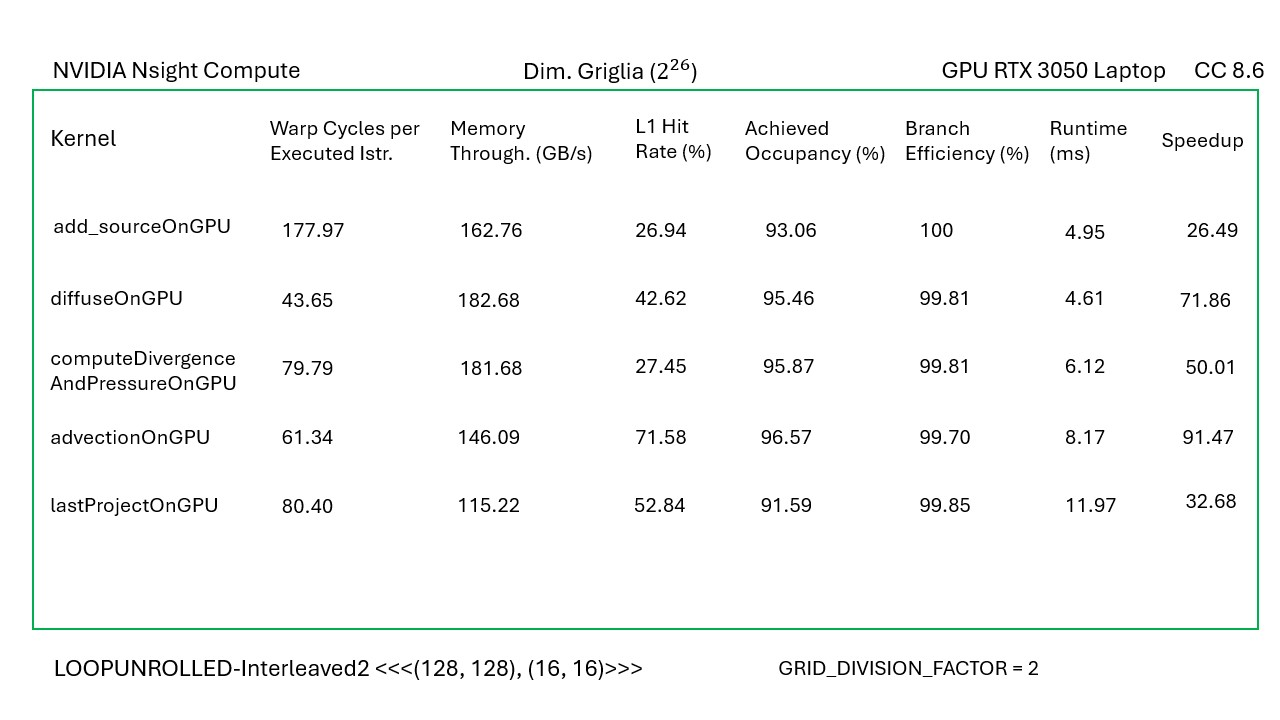
\includegraphics[width=0.75\linewidth]{figures/Slide9.jpg}
    \caption{Statistiche codice parallelo \texttt{LOOPUNROLLED-Interleaved2}}
    \label{fig:9}
\end{figure}

Tuttavia, l'efficienza non sembra migliorare a causa della natura memory-bound dei kernel. Le statistiche raccolte con \texttt{Nsight Compute} mostrano infatti che, in media, i warp subiscono maggiori stall nell'attesa dei dati dalla memoria (\emph{long scoreboard stalls}).

%Per concludere, analizzando il Roofline Model di tutti i kernel, si evince che tutti sono memory bound, ma le performance giacciono sulla Bandwidth Roof, questa significa che per aumentare le performance si deve provare un approccio diverso 



%\clearpage{\pagestyle{empty}\clearpage}

%%%%%%%%%%%%%%%%%%%%%%%%%%%%%%%%%%%%%%%%
% ANALISI E STUDIO PRESTAZIONI
\section{Analisi dei Risultati}
%Descrivete e inserite qui gli esperimenti effettuati e i dati raccolti. Se avete grafici e dati, presentateli in questa sezione (nella forma in cui pensate sia pi\`u facile visualizzare quello che volete far trasparire dai dati). Scrivete sempre su che supporti hardware o software avete effettuato le prove e quante ne avete fatte (se rilevante).

\subsection{Studio delle Prestazioni su Diversi Dataset}
%Prendendo in considerazione l'ultima versione, si è cercato inoltre di valutare il comportamento dell'implementazione al variare delle dimensioni dei dati in input. Testare l'algoritmo con dataset di dimensioni significativamente diverse è fondamentale per caratterizzare completamente il suo comportamento e validare l'efficacia delle ottimizzazioni implementate. In Figura \ref{fig:10} e \ref{fig:11} sono riportate i tempi di runtime della versione sequenziale e del \texttt{LOOPUNROLLED-Interleaved2}.

\begin{figure}
    \centering
    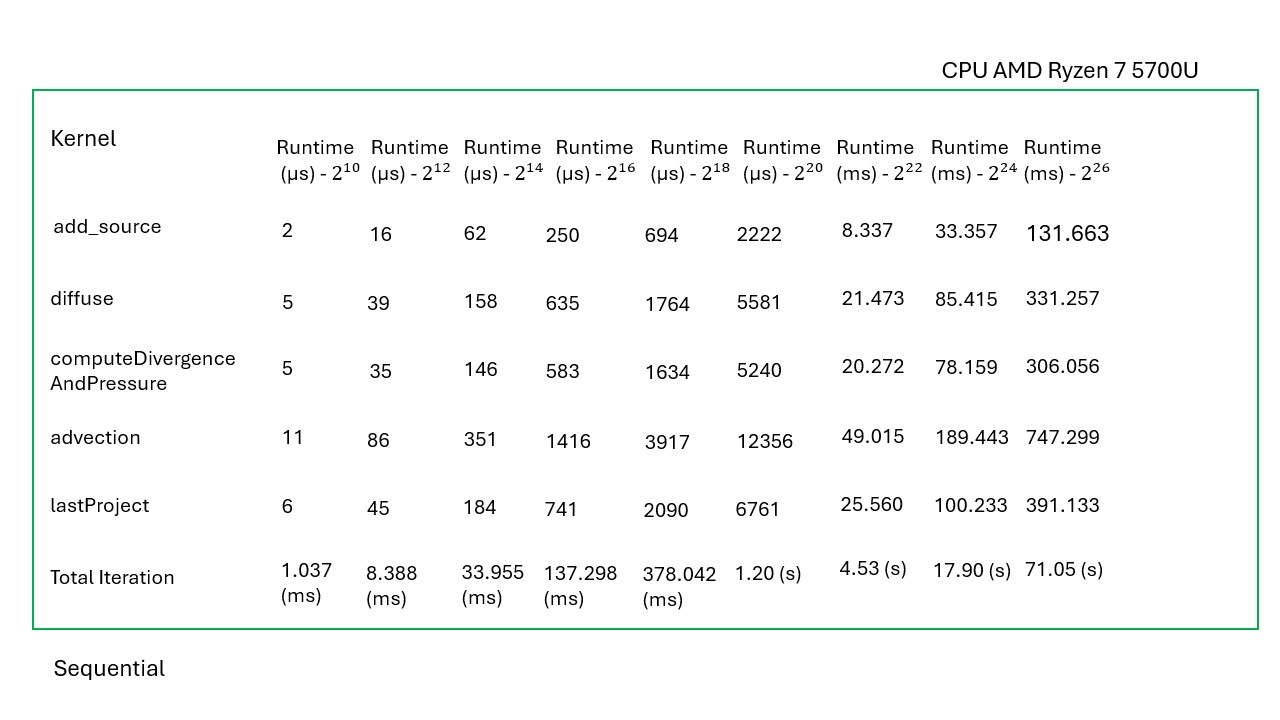
\includegraphics[width=0.75\linewidth]{figures/Slide11.jpg}
    \caption{Runtime codice sequenziale}
    \label{fig:10}
\end{figure}

Per valutare l'efficacia dell'implementazione, è stato analizzato il comportamento dell'algoritmo al variare delle dimensioni dei dataset in input. Testare l'algoritmo con dataset di dimensioni significativamente diverse è fondamentale per caratterizzarne il comportamento e validare l'efficacia delle ottimizzazioni implementate. In Figura \ref{fig:10} e \ref{fig:11} sono riportati i tempi di esecuzione della versione sequenziale e della versione ottimizzata \texttt{LOOPUNROLLED-Interleaved2}.


Già con \(2^{18}\) elementi, si osserva un significativo speedup, che aumenta linearmente all'aumentare delle dimensioni dei dati.

\subsubsection{Scelta del Tipo di Dato}

\begin{figure}
    \centering
    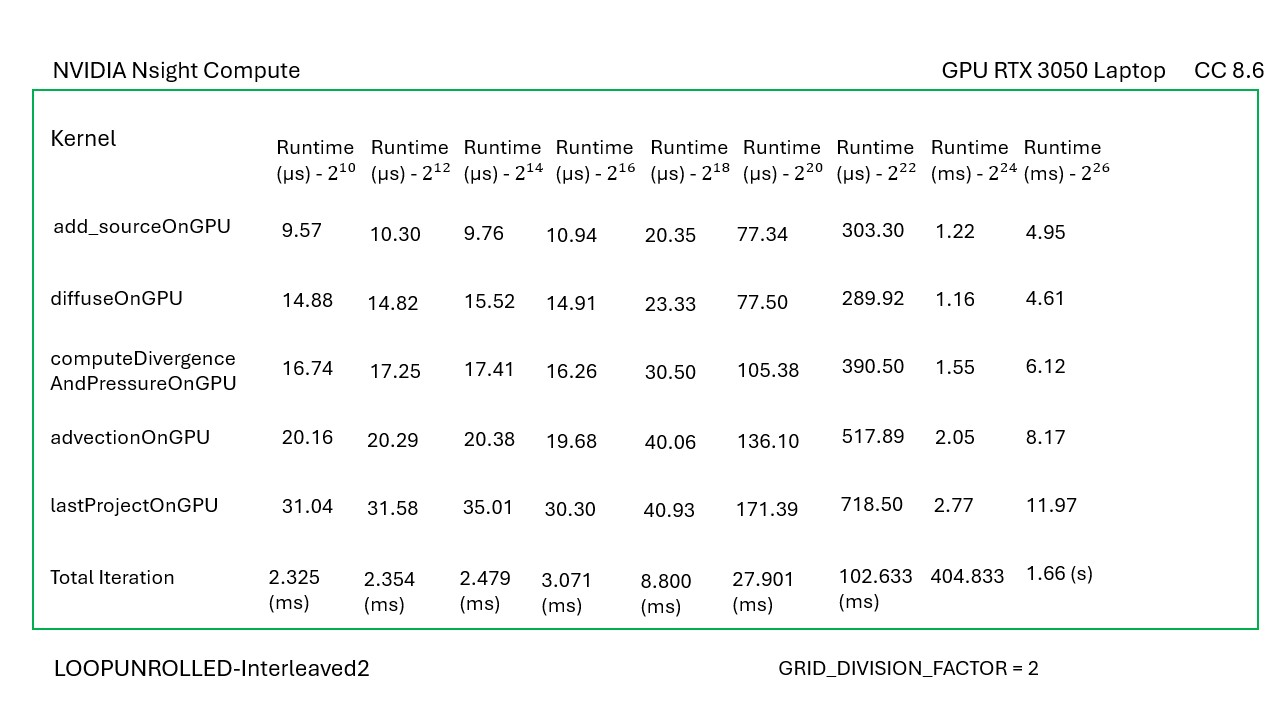
\includegraphics[width=0.75\linewidth]{figures/Slide10.jpg}
    \caption{Runtime codice parallelo \texttt{LOOPUNROLLED-Interleaved2}}
    \label{fig:11}
\end{figure}

Per questa implementazione, è stato preferito l'uso di variabili di tipo \texttt{float} anziché \texttt{double}. Questa scelta è motivata da diversi fattori:
\begin{itemize}
    \item I \texttt{float} richiedono meno memoria (la metà rispetto ai \texttt{double}), consentendo un utilizzo più efficiente della cache e delle unità di calcolo.
    \item Nel contesto della computer graphics, piccole imprecisioni numeriche sono meno critiche rispetto a un'applicazione ingegneristica. Pertanto, è stato privilegiato il guadagno in efficienza rispetto alla massima precisione.
    \item L'accuratezza tra la versione sequenziale e quella parallela è risultata comunque molto elevata, con una differenza nell'ordine di \(1 \times 10^{-6}\).
\end{itemize}

\subsubsection{Considerazioni sul Time Step}
Un altro aspetto rilevante è la scelta del time step per la simulazione. Con un time step di \(0.016s\), è possibile raggiungere una frequenza di circa \(62\) fps (frames per second). Tuttavia, per dataset di dimensioni maggiori, il tempo di calcolo supera questa soglia, rendendo necessario aumentare il time step per evitare che la simulazione appaia rallentata. Il numero massimo di elementi per cui la computazione rimane inferiore a \(0.016s\) è stato determinato empiricamente ed è pari a \(2^{18}\).

\subsection{Conclusioni Finali}
In conclusione, le versioni parallele dell'algoritmo hanno dimostrato un significativo miglioramento delle prestazioni, raggiungendo uno speedup considerevole. Tuttavia, per ulteriori ottimizzazioni, sarebbe opportuno esplorare approcci alternativi, come l'adozione di metodi più avanzati per la parallelizzazione o l'ottimizzazione della gestione della memoria. Infatti, metodi più sofisticati come il \textit{conjugate gradient} \cite{10.1145/882262.882364} e \textit{multigrid methods} \cite{10.1145/1198555.1198784, 10.1145/1198555.1198795} convergono più rapidamente rispetto al metodo di Jacobi, aumentando quindi l'efficienza.

%\subsubsection{Tipi di dato}
%Per questa implementazione si è preferito usare i float al posto dei double. Questo perché i float richiedono meno memoria (metà dei double), e consentono un uso più intensivo della cache e delle unità di calcolo. Infine, considerando che l'implementazione è rivolta al contesto della compputer graphics, imprecisioni al risultato finale non sono rilevanti tanto quanto in una applicazione ingegneristica, preferendo quindi efficienza rispetto a una precisione maggiore.
%Nel risultato, l'accuratezza tra la versione sequenziale e parallela è pari a (\(1e^-6\)).

%\subsubsection{Time step}
%Un altra considerazione riguarda il time-step dell'applicazione. Considerando un time step di \(0.016s\), si può arrivare a \(\frac{1}{0.016} \approx 62 \space \text{fps}\). Considerando che il maggior numero di elementi per cui la computazione richiede meno di \(0.016s\) è \(2^18\), per dati maggiori si deve prendere un timestep maggiore, per non far sembrare andare al rallentatore la simulazione.


%\subsection{Conclusioni Finali}
%Per concludere, le versioni parallele riescono a raggiungere un buon speedup con alte livelli di prestazioni. Tuttavia, se si volesse continuare a rendere più efficiente il programma, gli sforzi implementativi dovrebbe essere rivolti a un diverso metodo di risoluzione della \textbf{diffusione}. Infatti, metodi più sofisticati come il \textit{conjugate gradient} \cite{10.1145/882262.882364} e \textit{multigrid methods} \cite{10.1145/1198555.1198784, 10.1145/1198555.1198795} convergono con meno iterazioni rispetto al metodo di Jacobi.





\clearpage{\pagestyle{empty}\clearpage}

%%%%%%%%%%%%%%%%%%%%%%%%%%%%%%%%%%%%%%%%
% RISULTATI
%\section{Risultati}
%Descrivete e inserite qui gli esperimenti effettuati e i dati raccolti. Se avete grafici e dati, presentateli in questa sezione (nella forma in cui pensate sia pi\`u facile visualizzare quello che volete far trasparire dai dati). Scrivete sempre su che supporti hardware o software avete effettuato le prove e quante ne avete fatte (se rilevante).


%\clearpage{\pagestyle{empty}\clearpage}



%%%%%%%%%%%%%%%%%%%%%%%%%%%%%%%%%%%%%%%%
% CONCLUSIONI
%\chapter{Conclusioni e sviluppi futuri}

%Da scrivere alla fine, un breve riassunto di cosa si \`e affrontato, i risultati (se quanto indicato nell'introduzione come obiettivo \`e stato raggiunto) e come \`e possibile continuare la tesi (p.e. se qualcosa non \`e stato affrontato per motivi di tempo o limitazioni hardware).


%\clearpage{\pagestyle{empty}\clearpage}

%%%%%%%%%%%%%%%%%%%%%%%%%%%%%%%%%%%%%%%%%
% BIBLIOGRAFIA
\addcontentsline{toc}{chapter}{Bibliografia}
\label{Bibliography}
\bibliographystyle{IEEEtran}
\bibliography{src/bibliography}
\rhead[\fancyplain{}{\bfseries Bibliografia}]
{\fancyplain{}{\bfseries\thepage}}
\end{document}

